\documentclass{article}
\usepackage{graphicx}% http://ctan.org/pkg/graphicx
\usepackage{array}% http://ctan.org/pkg/array
\usepackage[table]{xcolor}
\newcolumntype{+}{>{\global\let\currentrowstyle\relax}}
\newcolumntype{^}{>{\currentrowstyle}}
\newcommand{\rowstyle}[1]{\gdef\currentrowstyle{#1}%
#1\ignorespaces
}
\begin{document}



\begin{table}[htb]
 \centering
\setlength{\arrayrulewidth}{.6mm}
\setlength{\tabcolsep}{5pt}
\renewcommand{\arraystretch}{.8}

 %\arrayrulecolor{blue}

  \begin{tabular}{  c | m{3cm} | m{3cm} | m{3cm} | m{1cm} }
    \hline
\rowcolor{lightgray}
\rowstyle{\bfseries}
%%%%%%First Row



    Microrobot Image & Type & Mathematical Model & Fabrication Method & Citation\\ \hline\hline
    \begin{minipage}{.3\textwidth}
      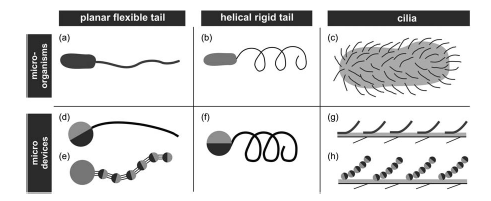
\includegraphics[width=\linewidth, height=20mm]{cilia}
    \end{minipage}
    &
     \begin{itemize}
        \item Accessibility
        \item Up to date information
        \item Fulfil students needs and wants \ldots
      \end{itemize}
    
    & 

      \begin{itemize}
        \item Accessibility
        \item Up to date information
        \item Fulfil students needs and wants \ldots
      \end{itemize}
    &

	 \begin{itemize}
        \item Accessibility
        \item Up to date information
        \item Fulfil students needs and wants \ldots
      \end{itemize} \\
%%%%%%Second Row
    \begin{minipage}{.3\textwidth}
      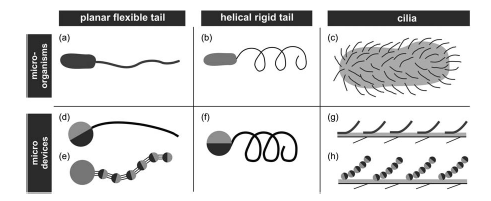
\includegraphics[width=\linewidth, height=20mm]{cilia}
    \end{minipage}
    &
     \begin{itemize}
        \item Accessibility
        \item Up to date information
        \item Fulfil students needs and wants \ldots
      \end{itemize}
    
    & 

      \begin{itemize}
        \item Accessibility
        \item Up to date information
        \item Fulfil students needs and wants \ldots
      \end{itemize}
    &

	 \begin{itemize}
        \item Accessibility
        \item Up to date information
        \item Fulfil stu
	 \end{itemize} \\

%%%%%%Third Row
 \begin{minipage}{.3\textwidth}
      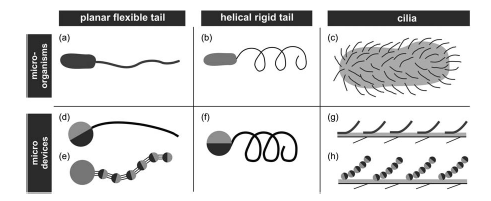
\includegraphics[width=\linewidth, height=20mm]{cilia}
    \end{minipage}
    &
     \begin{itemize}
        \item Accessibility
        \item Up to date information
        \item Fulfil students needs and wants \ldots
      \end{itemize}
    
    & 

      \begin{itemize}
        \item Accessibility
        \item Up to date information
        \item Fulfil students needs and wants \ldots
      \end{itemize}
    &

	 \begin{itemize}
        \item Accessibility
        \item Up to date information
        \item Fulfil students needs and wants \ldots
      \end{itemize} \\

%%%%%%Forth Row
 \begin{minipage}{.3\textwidth}
      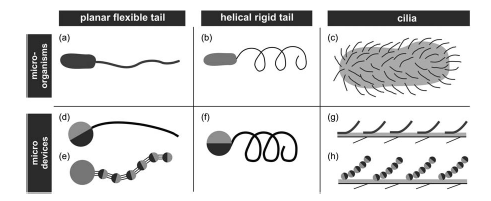
\includegraphics[width=\linewidth, height=20mm]{cilia}
    \end{minipage}
    &
     \begin{itemize}
        \item Accessibility
        \item Up to date information
        \item Fulfil students needs and wants \ldots
      \end{itemize}
    
    & 

      \begin{itemize}
        \item Accessibility
        \item Up to date information
        \item Fulfil students needs and wants \ldots
      \end{itemize}
    &

	 \begin{itemize}
        \item Accessibility
        \item Up to date information
        \item Fulfil students needs and wants \ldots
      \end{itemize} \\

%%%%%%Fifth Row
 \begin{minipage}{.3\textwidth}
      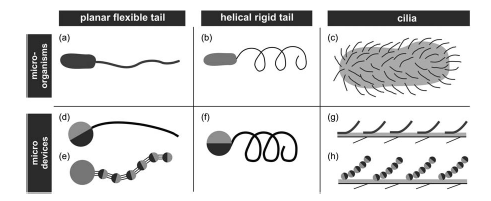
\includegraphics[width=\linewidth, height=20mm]{cilia}
    \end{minipage}
    &
     \begin{itemize}
        \item Accessibility
        \item Up to date information
        \item Fulfil students needs and wants \ldots
      \end{itemize}
    
    & 

      \begin{itemize}
        \item Accessibility
        \item Up to date information
        \item Fulfil students needs and wants \ldots
      \end{itemize}
    &

	 \begin{itemize}
        \item Accessibility
        \item Up to date information
        \item Fulfil students needs and wants \ldots
      \end{itemize} 


    \\ \hline
  \end{tabular}
  \caption{my.Lboro Analysis}\label{tbl:myLboro}

\end{table}





\end{document}